\documentclass{standalone}

\usepackage{tikz,fp}
\usetikzlibrary{calc}
\usetikzlibrary{decorations.markings}

\tikzset{>=stealth,
  coord/.style = {circle,fill=black,draw=black,minimum size=0.1cm,inner sep=0pt},
  tangent/.style={decoration={markings, mark= at position #1
      with{
        \coordinate (tangent point-\pgfkeysvalueof{/pgf/decoration/mark info/sequence number})
                                     at (0pt,0pt);
        \coordinate (tangent unit vector-\pgfkeysvalueof{/pgf/decoration/mark info/sequence number}) at (1,0pt);
        \coordinate (tangent orthogonal unit vector-\pgfkeysvalueof{/pgf/decoration/mark info/sequence number}) at (0pt,1);
      }
    },
    postaction=decorate
  },
  use tangent/.style={shift=(tangent point-#1), x=(tangent unit vector-#1),
    y=(tangent orthogonal unit vector-#1)},
  use tangent/.default=1
}

\makeatletter
\def\calcLength(#1,#2)#3{%
\pgfpointdiff{\pgfpointanchor{#1}{center}}%
             {\pgfpointanchor{#2}{center}}%
\pgf@xa=\pgf@x%
\pgf@ya=\pgf@y%
\FPeval\@temp@a{\pgfmath@tonumber{\pgf@xa}}%
\FPeval\@temp@b{\pgfmath@tonumber{\pgf@ya}}%
\FPeval\@temp@sum{(\@temp@a*\@temp@a+\@temp@b*\@temp@b)}%
\FProot{\FPMathLen}{\@temp@sum}{2}%
\FPround\FPMathLen\FPMathLen5\relax
\global\expandafter\edef\csname #3\endcsname{\FPMathLen}
}
\makeatother

\usepackage{xcolor}

\begin{document}
\pagecolor{white}

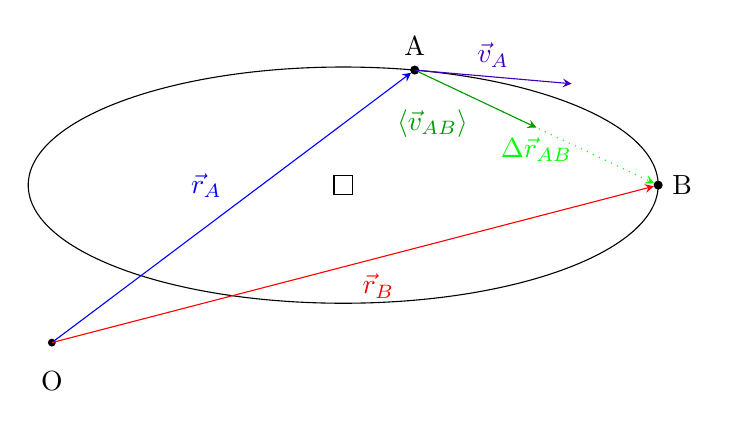
\begin{tikzpicture}
  \def\start{0.2}
  \def\stop{0}
  \def\diff{\start - \stop}
  \def\speed{2}
  \coordinate (O) at (0,0);
  \coordinate (C) at (3.7,2);
  \draw[tangent = \start, tangent = \stop] (C) ellipse (4 and 1.5);
  \node[use tangent,coord] (A) at (0,0) {};
  \node [above] at (A.north) {A};
  \node[use tangent=2,coord] (B) at (0,0) {};
  \node [right] at (B.east) {B};

  \calcLength(A,B){disp};
  \node at (C)[draw] {\disp};

  \fill (O) circle (0.05) node [below=0.25cm]{O};

  \draw[blue,->] (O) -- (A) node[midway, above left]{$\vec{r}_A$};
  \draw[red,->] (O) -- (B) node[midway, below right]{$\vec{r}_B$};
  \draw[green,dotted,->] (A) -- (B) node[midway, below]{$\Delta\vec{r}_{AB}$};
  \draw[green!60!black,->] (A) -- ($(A)!0.5!(B)$)
          node[midway, below left]{$\langle\vec{v}_{AB}\rangle$};
  

  \draw[blue!50!violet, ->, use tangent] (0,0) -- (-\speed,0) node[midway,above]{$\vec{v}_A$};
\end{tikzpicture}
\end{document}